%=========================================================
% Interrupts and INTC 
%=========================================================
\section{Interrupts and INTC (Interrupt Controller)}

The mmRISC-1 supports the following four interrupt request inputs. 

\begin{description}
    \item[IRQ\_EXT] External Interrupt
    \item[IRQ\_MSOFT] Machine Software Interrupt IRQ\_MTIME Machine Timer Interrupt
    \item[{IRQ[63:0]}] Interrupt Request (towards Interrupt Controller)
\end{description}

Priority among above interrupts is defined as IRQ\_EXT > IRQ\_SOFT > IRQ\_MTIME > IRQ[63:0].
64 IRQ inputs are controlled by INTC (Interrupt Controller) shown in Figure \ref{fig:INTERRUPTS_INTC}. The INTC can be configured by dedicated CSRs. INTCFGSENSE0/1 select each IRQ sense way from level sense or rising edge sense. INTPENDING0/1 show each IRQ input logic level for level sense, or pending status for rising edge sense. For rising edge IRQ, pending status can be cleared by writing 1 to each corresponding bit. INTCFGENABLE0/1 enable or disable each interrupt.\\

INTCFGPRIORITY0/1/2/3 configure priority level of each IRQ. The priority level is expressed in 4bits, 4’b0000 is lowest and 4’b1111 is highest. In priority tournament block, one IRQ having the highest priority level is selected from requesting IRQ, and finally if the priority is larger than MINTCURLVL, the selected IRQ is outputted. When CPU accepts the IRQ request, MINTCURLVL is automatically transferred to MINTPRELVL, and priority level of accepted IRQ is also automatically transferred to MINTCURLVL. In last phase of interrupt software handler before MRET, software should copy MINTPRELVL to MINTCURLVL. Thus IRQ allows nested interrupts.

\begin{figure}[H]
    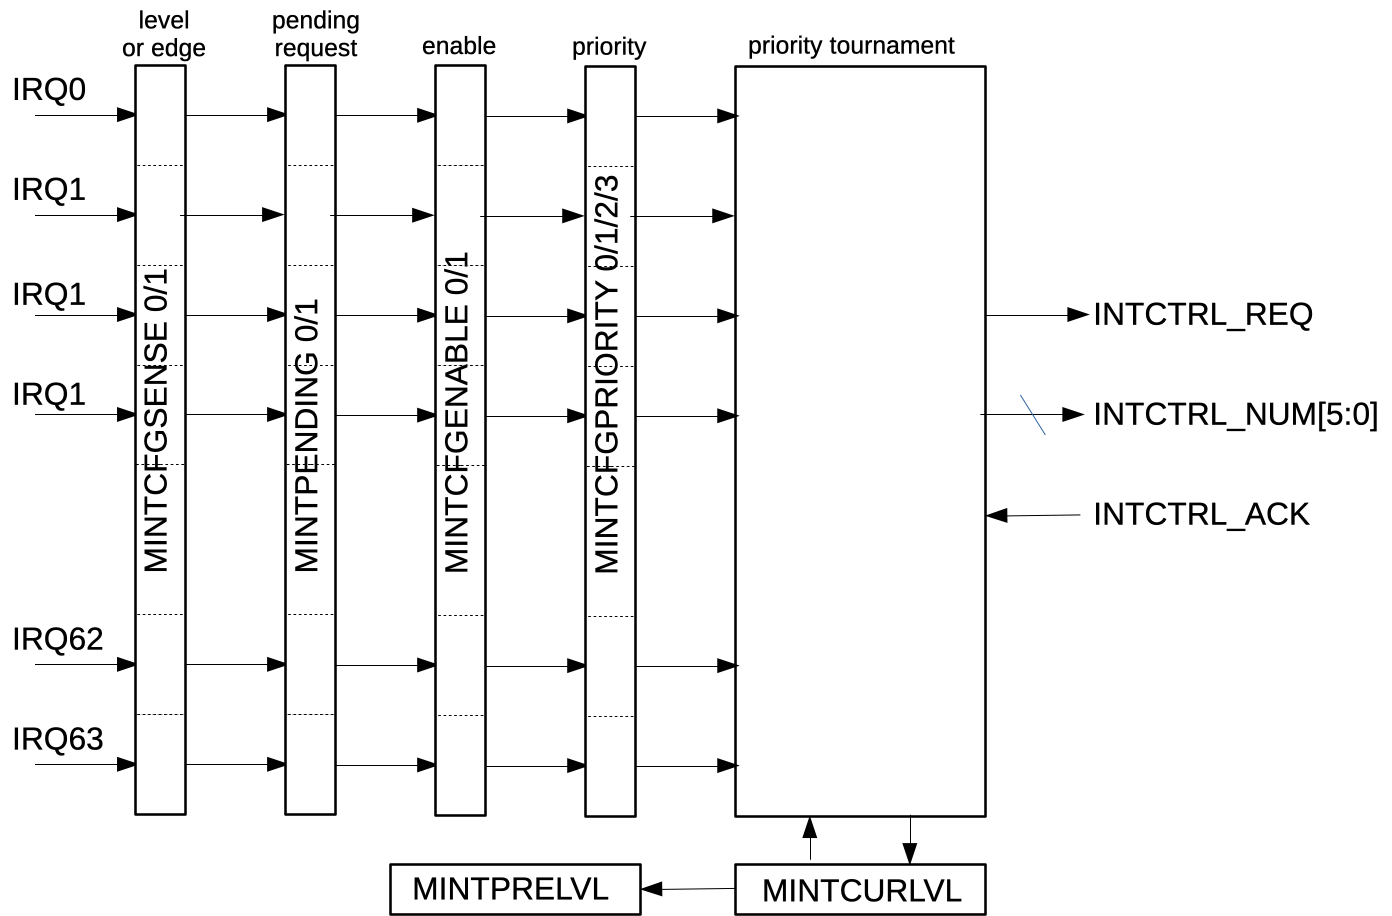
\includegraphics[width=1.00\columnwidth]{./Figure/Interrupts_INTC.png}
    \caption{INTC (Interrupt Controller)}
    \label{fig:INTERRUPTS_INTC}
\end{figure}

An example of a startup routine that includes exception handlers and interrupt entry points is shown in Listing \ref{list:STARTUPROUTINE}. Also, an example of interrupt initialization routines and interrupt handler routines written in C language, which are combined with the startup routine, are shown in Listing \ref{list:INTERRUPTCROUTINE}. The sample routines support nested interrupts.

The sample routine depends on the GNU C compiler to save and restore the XRn and FRn registers by using the keyword "\_\_attribute\_\_ ((interrupt))" to define the interrupt handler routines. 

In this example, multiple interrupts with different priorities are gathered into one entry point and one handler routine "INT\_Handler\_IRQ()". This example increases the interrupt latency due to the conditional judgment in the handler routine.

If you want to improve the latency of each interrupt, it is recommended to prepare pairs of dedicated entry point and corresponding handler routine for each interrupt as shown in \ref{list:DEDICATEDHANDLER}. In the case, the interrupt nesting is not supported.


%-------------------
\begin{lstlisting}[caption=An Example of Startup Routine including Exception Handlers and Interrupt Entry Points written in Assembler language, captionpos=b, language=, frame=single, basicstyle=\ttfamily\scriptsize, label=list:STARTUPROUTINE]
    .globl _start
    .globl main
    .globl INT_Handler_EXT
    .globl INT_Handler_MSOFT
    .globl INT_Handler_MTIME
    .globl INT_Handler_IRQ
//-----------------------------------
// Reset Vector
//-----------------------------------
    .text
    .section ".vectors"
    .align 4
_reset:
    j    _start
_vector_base:
    j    _trap_exception       // 00:Exception
    j    _trap_illegal         // 01:Supervisor Software Interrupt
    j    _trap_illegal         // 02:Reserved
    j    INT_Handler_MSOFT     // 03:Machine Software Interrupt
    j    _trap_illegal         // 04:Reserved
    j    _trap_illegal         // 05:Reserved
    j    _trap_illegal         // 06:Reserved
    j    INT_Handler_MTIME     // 07:Machine Timer Interrupt
    j    _trap_illegal         // 08:Reserved
    j    _trap_illegal         // 09:Reserved
    j    _trap_illegal         // 10:Reserved
    j    INT_Handler_EXT       // 11:Machine External Interrupt
    j    _trap_illegal         // 12:Reserved
    j    _trap_illegal         // 13:Reserved
    j    _trap_illegal         // 14:Reserved
    j    _trap_illegal         // 15:Reserved
    j    INT_Handler_IRQ       // 16:IRQ00
    j    INT_Handler_IRQ       // 17:IRQ01
    j    INT_Handler_IRQ       // 18:IRQ02
    j    INT_Handler_IRQ       // 19:IRQ03
    ...
    j    INT_Handler_IRQ       // 76:IRQ60
    j    INT_Handler_IRQ       // 77:IRQ61
    j    INT_Handler_IRQ       // 78:IRQ62
    j    INT_Handler_IRQ       // 79:IRQ63

//-----------------------------------
// Trap Entry
//-----------------------------------
    .text
    .section ".trap"
    .align 4
//
_trap_exception:
   // Do Nothing
    mret
//
_trap_illegal:
   // Forever Loop as a Trap
   j     .

//--------------------------------
// Startup
//--------------------------------
    .text
    .section ".startup"
_start:
    //
    // Init GP and SP
    la  gp, __GLOBAL_PTR__
    la  sp, __STACK_TOP__
    //
    // Copy Initial Data
    la  a0, __ROM_INIT_BGN__
    la  a1, __RAM_INIT_BGN__
    la  a2, __RAM_INIT_END__
    bgeu a1, a2, 2f
1:
    lw t0, (a0)
    sw t0, (a1)
    addi a0, a0, 4
    addi a1, a1, 4
    bltu a1, a2, 1b
2:
    //
    // Clear BSS
    la a0, __BSS_BGN__
    la a1, __BSS_END__
    bgeu a0, a1, 2f
1:
    sw zero, (a0)
    addi a0, a0, 4
    bltu a0, a1, 1b
2:
    //
    // Setup MTVEC
    la   t0, _vector_base
    ori  t0, t0, 0x01 // vectored
    csrw mtvec, t0
    //
    // Goto Main
    call main
    //
    // Forever Loop
3:
    j    3b
\end{lstlisting}
%------------------------------------------
\begin{lstlisting}[caption=An Example of Interrupt Initializations and Interrupt Handlers written in C language, captionpos=b, language=, frame=single, basicstyle=\ttfamily\scriptsize, label=list:INTERRUPTCROUTINE]
#include <stdint.h>
#include "common.h"
#include "csr.h"
#include "gpio.h"
#include "system.h"
#include "uart.h"
#include "interrupt.h"

//--------------------------
// Interrupt Initialization
//--------------------------
void INT_Init(void)
{
    uint32_t irq;
    uint32_t level;
    //
    // Configure IRQ00 as UART RXD Interrupt
    IRQ_Config(0, 1, 1, 1);
    //
    // Enable MTIME to make periodic interrupt
    MTIME_Init(1, 10, 1, 0, 166666); // 100ms
    //
    // Enable MTIME and IRQ Interrupts
    INT_Config(0, 1, 0, 1, 0x0);
}

//--------------------------
// IRQ Configuration
//--------------------------
void IRQ_Config
(
    uint32_t irqnum,   // IRQ Number : 0 ~ 63
    uint32_t enable,   // IRQ Enable : 0=Disable, 1=Enable
    uint32_t sense,    // IRQ Sense  : 0=Level  , 1=Edge
    uint32_t level     // IRQ Level  : 0 ~ 15
)
{
    uint32_t pos1, pos4;
    uint32_t data;
    //
    enable = enable & 0x01;
    sense  = sense  & 0x01;
    level  = level & 0x0f;
    //
    // Set Priority
    if (irqnum < 8)
    {
        pos4 = (irqnum - 0) * 4;
        //
        data = read_csr(MINTCFGPRIORITY0);
        data = (data & ~(0x0f << pos4)) | (level << pos4);
        write_csr(MINTCFGPRIORITY0, data);
    }
    else if (irqnum < 16)
    {
        pos4 = (irqnum - 8) * 4;
        //
        data = read_csr(MINTCFGPRIORITY1);
        data = (data & ~(0x0f << pos4)) | (level << pos4);
        write_csr(MINTCFGPRIORITY1, data);
    }
    else if (irqnum < 24)
    {
        pos4 = (irqnum - 16) * 4;
        //
        data = read_csr(MINTCFGPRIORITY2);
        data = (data & ~(0x0f << pos4)) | (level << pos4);
        write_csr(MINTCFGPRIORITY2, data);
    }
    else if (irqnum < 32)
    {
        pos4 = (irqnum - 24) * 4;
        //
        data = read_csr(MINTCFGPRIORITY3);
        data = (data & ~(0x0f << pos4)) | (level << pos4);
        write_csr(MINTCFGPRIORITY3, data);
    }
    else if (irqnum < 40)
    {
        pos4 = (irqnum - 32) * 4;
        //
        data = read_csr(MINTCFGPRIORITY4);
        data = (data & ~(0x0f << pos4)) | (level << pos4);
        write_csr(MINTCFGPRIORITY4, data);
    }
    else if (irqnum < 48)
    {
        pos4 = (irqnum - 40) * 4;
        //
        data = read_csr(MINTCFGPRIORITY5);
        data = (data & ~(0x0f << pos4)) | (level << pos4);
        write_csr(MINTCFGPRIORITY5, data);
    }
    else if (irqnum < 56)
    {
        pos4 = (irqnum - 48) * 4;
        //
        data = read_csr(MINTCFGPRIORITY6);
        data = (data & ~(0x0f << pos4)) | (level << pos4);
        write_csr(MINTCFGPRIORITY6, data);
    }
    else if (irqnum < 64)
    {
        pos4 = (irqnum - 56) * 4;
        //
        data = read_csr(MINTCFGPRIORITY7);
        data = (data & ~(0x0f << pos4)) | (level << pos4);
        write_csr(MINTCFGPRIORITY7, data);
    }
    //
    // Set Sense and Enable
    if (irqnum < 32)
    {
        pos1 = (irqnum - 0);
        //
        data = read_csr(MINTCFGSENSE0);
        data = (data & ~(0x01 << pos1)) | (sense << pos1);
        write_csr(MINTCFGSENSE0, data);
        //
        data = read_csr(MINTCFGENABLE0);
        data = (data & ~(0x01 << pos1)) | (enable << pos1);
        write_csr(MINTCFGENABLE0, data);
    }
    else if (irqnum < 64)
    {
        pos1 = (irqnum - 32);
        //
        data = read_csr(MINTCFGSENSE1);
        data = (data & ~(0x01 << pos1)) | (sense << pos1);
        write_csr(MINTCFGSENSE1, data);
        //
        data = read_csr(MINTCFGENABLE1);
        data = (data & ~(0x01 << pos1)) | (enable << pos1);
        write_csr(MINTCFGENABLE1, data);
    }
}

//--------------------------
// Interrupt Configuration
//--------------------------
void INT_Config
(
    uint32_t ena_intext,   // Enable External Interrupt
    uint32_t ena_intmtime, // Enable MTIME Interrupt
    uint32_t ena_intmsoft, // Enable SOFTWARE Interrupt
    uint32_t ena_irq,      // Enable IRQ Interrupts
    uint32_t cur_irqlvl    // Current IRQ Level
)
{
    uint32_t data;
    //
    ena_intext   = ena_intext & 0x01;
    ena_intmtime = ena_intmtime & 0x01;
    ena_intmsoft = ena_intmsoft & 0x01;
    ena_irq      = ena_irq & 0x01;
    cur_irqlvl   = cur_irqlvl & 0x0f;
    //
    // Interrupt Current Level
    write_csr(MINTCURLVL, cur_irqlvl);
    //
    // Enable Interrupt
    data = read_csr(MIE);
    data = (data & ~((1<<11) | (1<<7)| (1<<3)))
         | (ena_intext << 11) | (ena_intmtime << 7) | (ena_intmsoft << 3);
    write_csr(MIE, data);
    //
    data = read_csr(MSTATUS);
    data = (data & ~(0x01 << 3))
         | ((ena_intext | ena_intmtime | ena_intmsoft | ena_irq) << 3);
    write_csr(MSTATUS, data);
}

//---------------------------
// Interrupt Generate
//---------------------------
void INT_Generate
(
    uint32_t intext,
    uint32_t intsoft,
    uint64_t irq
)
{
    mem_wr32(INTGEN_IRQ_EXT, intext  & 0x01);
    mem_wr32(MSOFTIRQ      , intsoft & 0x01);
    mem_wr32(INTGEN_IRQ1   , (uint32_t)(irq >> 32));
    mem_wr32(INTGEN_IRQ0   , (uint32_t)(irq & 0x0ffffffffUL));
}

//---------------------
// MTIME Initialization
//---------------------
void MTIME_Init
(
    uint32_t enable,
    uint32_t div_plus_one,
    uint64_t intena,
    uint64_t mtime_count,
    uint64_t mtime_compa
)
{
    uint32_t div;
    //
    enable = enable & 0x01;
    div    = (div_plus_one > 0)? div_plus_one - 1 : div_plus_one;
    div    = div & 0x3f;
    intena = intena & 0x01;
    //
    mem_wr32(MTIME_DIV , div);
    mem_wr32(MTIME     , (uint32_t)(mtime_count & 0x0ffffffffUL));
    mem_wr32(MTIMEH    , (uint32_t)(mtime_count >> 32          ));
    mem_wr32(MTIMECMP  , (uint32_t)(mtime_compa & 0x0ffffffffUL));
    mem_wr32(MTIMECMPH , (uint32_t)(mtime_compa >> 32          ));
    mem_wr32(MTIME_CTRL, (intena << 2) | (enable << 0));
}

//-----------------------------
// Interrupt Handler External
//-----------------------------
__attribute__ ((interrupt)) void INT_Handler_EXT(void)
{
    // Negate IRQ_EXT
    mem_wr32(INTGEN_IRQ_EXT, 0x00000000);
    //
    // Write your own code
    ...
}

//----------------------------
// Interrupt Handler MTIME
//----------------------------
__attribute__ ((interrupt)) void INT_Handler_MTIME(void)
{
    // Clear Interrupt Flag in MTIME
    mem_wr32(MTIME_CTRL, mem_rd32(MTIME_CTRL));
    //
    // Write your own code
    ...
}

//-----------------------------
// Interrupt Handler MSOFT
//-----------------------------
__attribute__ ((interrupt)) void INT_Handler_MSOFT(void)
{
    // Negate MSOFT
    mem_wr32(MSOFTIRQ, 0x00000000);
    //
    // Write your own code
    ...
}

//-------------------------
// Interrupt Handler IRQ
//-------------------------
__attribute__ ((interrupt)) void INT_Handler_IRQ(void)
{
    uint32_t irq_level;
    uint64_t irq_pend0;
    uint64_t irq_pend1;
    uint64_t irq_pend;
    uint32_t prev_mepc;
    uint32_t prev_mstatus;
    uint32_t prev_mintprelvl;
    //
    // Get Pending Status
    irq_level = read_csr(MINTCURLVL);
    irq_pend0 = (uint64_t)read_csr(MINTPENDING0);
    irq_pend1 = (uint64_t)read_csr(MINTPENDING1);
    irq_pend  = (irq_pend1 << 32) + (irq_pend0 << 0);
    //
    // Save Previous Status
    prev_mintprelvl = read_csr(MINTPRELVL);
    prev_mepc       = read_csr(MEPC);
    prev_mstatus    = read_csr(MSTATUS);
    //
    // Enable global interrupt (set mie)
    write_csr(MSTATUS, prev_mstatus | 0x08);
    //
    //-------------------------------------------------
    // Dispatch to each Priority Handler
    switch(irq_level)
    {
        // Group Priority Level 1
        case  1 :
        {
            // Write your own code
            // IRQ00
            if (irq_pend0 & 0x00000001)
            {
                INT_UART_Handler();
                write_csr(MINTPENDING0, 0x00000001); // Clear Pending Edge
            }
            break;
        }
        // Group Priority 2-15
        case  2 :
        case  3 :
        case  4 :
        case  5 :
        case  6 :
        case  7 :
        case  8 :
        case  9 :
        case 10 :
        case 11 :
        case 12 :
        case 13 :
        case 14 :
        case 15 :
        {
            // Write your own code
            break;
        }
        //  Never reach here
        default :
        {
            break;
        }
    }
    //-------------------------------------------------
    //
    // Disable global interrupt, Save Previous Status
    write_csr(MSTATUS   , prev_mstatus); // mie=0
    write_csr(MEPC      , prev_mepc);
    write_csr(MINTCURLVL, prev_mintprelvl);
}
\end{lstlisting}

%-------------------
\begin{lstlisting}[caption=An Example of Interrupt related routines (assembler and C) involving pairs of dedicated entry point and corresponding handler routine in order to improve the interrupt latency, captionpos=b, language=, frame=single, basicstyle=\ttfamily\scriptsize, label=list:DEDICATEDHANDLER]
==== Assembler Part ====
...
_vector_base:
...
    j    INT_Handler_IRQ00     // 16:IRQ00
    j    INT_Handler_IRQ01     // 17:IRQ01
    j    INT_Handler_IRQ02     // 18:IRQ02
    j    INT_Handler_IRQ03     // 19:IRQ03
...

==== C language Part ====
...
__attribute__ ((interrupt)) void INT_Handler_IRQ00(void)
{
    // Write your own code
}
__attribute__ ((interrupt)) void INT_Handler_IRQ01(void)
{
    // Write your own code
}
__attribute__ ((interrupt)) void INT_Handler_IRQ02(void)
{
    // Write your own code
}
__attribute__ ((interrupt)) void INT_Handler_IRQ03(void)
{
    // Write your own code
}
...
\end{lstlisting}


